\documentclass[conference]{IEEEtran}
\usepackage{config/ieee-paper}
\usepackage{lipsum}
\hyphenation{
    % A
    %
    % B
    %
    % C
    %
    % D
    %
    % E
    %
    % F
    %
    % G
    %
    % H
    %
    % I
    % 
    % J
    %
    % K
    %
    % L
    %
    % M
    %
    % N
    %
    % O
    %
    % P
    %
    % Q
    %
    % R
    %
    % S
    %
    % T
    % 
    % U
    %
    % V
    %
    % W
    %
    % X
    %
    % Y
    % 
    % Z
    %
}
% Adding references to the document
\addbibresource{IEEEabrv.bib}
\addbibresource{references.bib}
\IEEEoverridecommandlockouts{}
% The preceding line is only needed to identify funding in the first footnote. If that is unneeded, please comment it out.
\begin{document}
\title{CSC730: Assignment 7\\Isolation Forests - Anomaly Detection by Isolating Anomalies}
\author{\IEEEauthorblockN{Kristophor Ray Jensen}
    \IEEEauthorblockA{\textit{Electrical Engineering and Computer Science} \\
        \textit{South Dakota School of Mines and Technology}\\
        Rapid City, United States \\
        0009-0001-7344-349X}

}
\maketitle
\section{Introduction}
%TODO: discussion of the problem and its significance
%TODO: description of active learning
%TODO: description of rare class discovery
%TODO: description of the datasets

The requirements for this assignment are as follows~\cite{assignment9}.\par
\begin{enumerate}    
    \item Get the provided datasets from D2L. Then for each dataset:
    \item Visualize the data w/ labels using 2 or 3-D tSNE.
    \item Write your own version of an active learning rare class discovery algorithm.
    \item Run your code on the dataset and keep track of the number of classes discovered vs. number of
    queries.
    \item Plot that (\# classes discovered vs. \# queries).
    \item Rerun the same experiment using a random query strategy.
    \item Plot the results from the random algorithm on the same plot.    
\end{enumerate}


\section{Methodology}

\subsection{Active Learning Algorithm Overview}
The main components of the active learning algorithm include the following~\cite{tharwat2023survey}:
\begin{itemize}
    \item \textbf{Dataset:} The dataset consists of labeled and unlabeled instances. The labeled instances are used to train the model, while the unlabeled instances are used to select instances for labeling.
    \item \textbf{Learning Algorithm:} The classifier is a machine learning model that is trained on the labeled data. The classifier is used to make predictions on the unlabeled data and select instances for labeling.    
    \item \textbf{Query Strategy:} The query strategy determines which instances to query for labels. The query strategy selects instances that the model is most uncertain about, based on the current model's predictions.        
    \item \textbf{Expert:} The expert is the user who provides labels for the selected instances. The expert labels the instances selected by the query strategy, and the labels are used to update the model.
\end{itemize}

\subsection{Dataset}
The MNIST data set consists of 70,000 labelled points. Each point is a 28x28 image of a digit from 0 to 9. 
The images are reshaped to a 1D array of length 784 and normalized to the range [0, 1]. 
The data set is balanced, with an equal number of images for each digit class. \par
In our example we created a 20\% split of the data set to be used as the test set. The training dataset was then put into a pool of unlabeled data.

A second list of the training data was created to be used as the labeled data. This method reminds of of the psuedo-labeling method used in semi-supervised learning that we recreated in assignment 4.\par

Figure~\ref{fig:nominal_train} shows a random selection of 16 nominal images from the training set.
\begin{figure}[htbp]
    \centering
    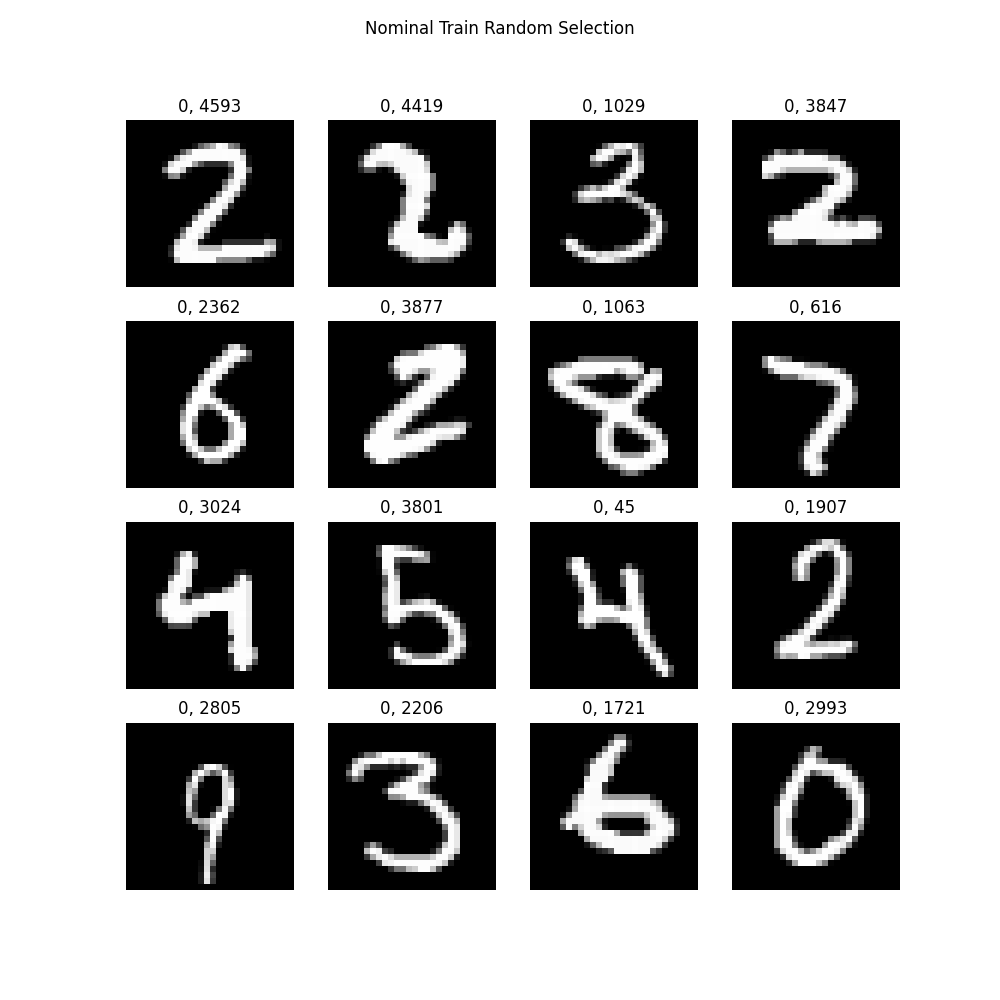
\includegraphics[width=0.5\textwidth]{resources/images/_nominal_train_random_selection.png}
    \caption{Random selection of nominal images from the training set}
    \label{fig:nominal_train}
    \end{figure}
\subsection{Learning Algorithm}
There were two classifiers used in this assignment. The first classifier was a random forest classifier, and the second classifier was a support vector machine (SVM) classifier.
The random forest classifier was used as the base classifier for the active learning algorithm. The SVM classifier was used to compare the performance of the active learning algorithm with a different classifier. 
The classifiers were trained on the labeled data and used to make predictions on the unlabeled data. The predictions were used to select instances for labeling based on the query strategy. 
The classifiers were updated with the newly labeled instances, and the process was repeated for either a maximum number of iterations or minimum single-class accuracy reaching a threshold of 95\%.


\subsection{Query strategy}
In this assignment, we implemented the following query strategies:
\begin{itemize}
    \item \textbf{Random Sampling:} Randomly select instances from the pool of unlabeled data for labeling. This strategy serves as a baseline for comparison with other query strategies.
    \item \textbf{Highest Confidence:} Select instances for labeling based on the classifier's highest confidence in its predictions. The highest confidence is calculated as the highest predicted probability for each instance.
    \item \textbf{Least Confidence:} Select instances for labeling based on the classifier's least confidence in its predictions. The least confidence is calculated as the difference between the highest and second-highest predicted probabilities for each instance.    
    \item \textbf{Entropy Sampling:} Select instances for labeling based on the classifier's entropy of confidence in its predictions. The entropy is calculated as the negative sum of the predicted probabilities for each instance.
    \item \textbf{Lowest Vote:} Select instances for labeling based on the classifier's lowest vote in its predictions. The lowest vote is calculated as the lowest predicted probability for each instance.
\end{itemize}

\subsection{Expert}
The expert in this assignment was simulated by selecting instances from the pool of unlabeled data for labeling. The instances were selected based on the query strategy, and the labels were used to update the model. The expert was assumed to provide accurate labels for the selected instances.


\subsection{Evaluation Metrics}
Confusion matrices and accuracy scores were used to evaluate the performance of the active learning algorithm. The confusion matrix shows the number of true positives, false positives, true negatives, and false negatives for each class.
The accuracy score is the proportion of correctly classified instances out of the total number of instances. The confusion matrix and accuracy score were calculated at each iteration of the active learning algorithm to track the performance of the model over time.

The probabilities from the data set are in the following output excerpt:
Probabilities for Each Class:
% \begin{center}    
%     \captionof{Probabilities for Each Class\label{tab:probabilities}}
%     \begin{tabular}{cc}
%         \hline
%         Class & Probability \\
%         \hline
%         3.0 & 0.5007 \\
%         4.0 & 0.2503 \\
%         9.0 & 0.1251 \\
%         6.0 & 0.0626 \\
%         2.0 & 0.0313 \\
%         0.0 & 0.0156 \\
%         5.0 & 0.0078 \\
%         8.0 & 0.0038 \\
%         1.0 & 0.0019 \\
%         7.0 & 0.0009 \\
%         \hline
%     \end{tabular}    
% \end{center}
%If we inspect the histogram of the incoming true classes we see the results in figure~\ref{fig:histogram}. 
%However, the results of the classification are shown in figure~\ref{fig:classification}.

\begin{center}    
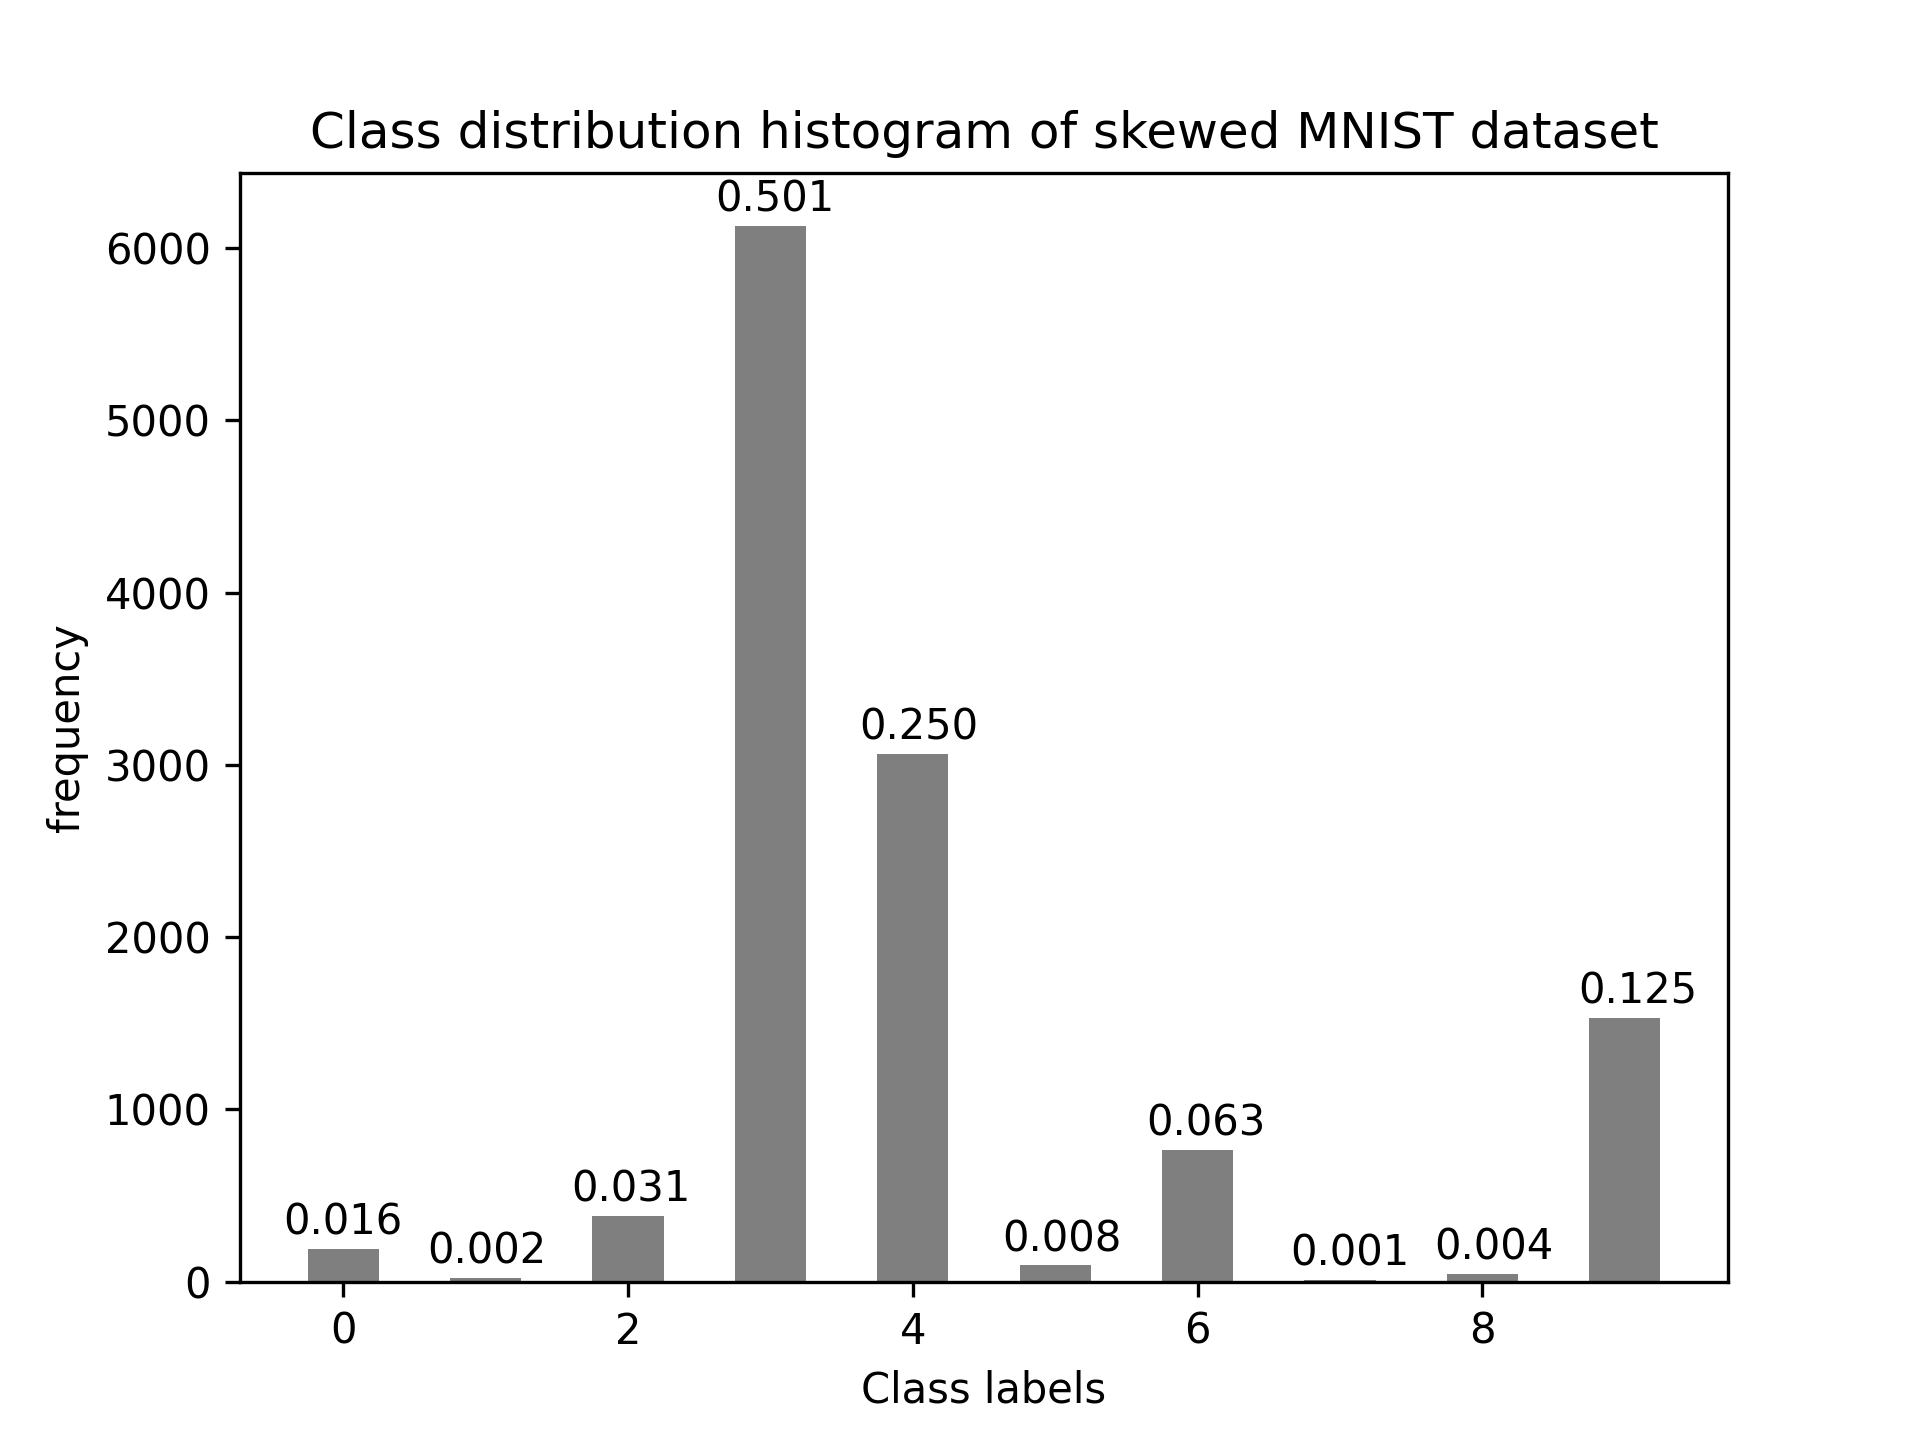
\includegraphics[width=0.5\textwidth]{class_histogram.png}
%\captionof{Histogram of True Classes\label{fig:histogram}}
\end{center}    


\begin{center}    
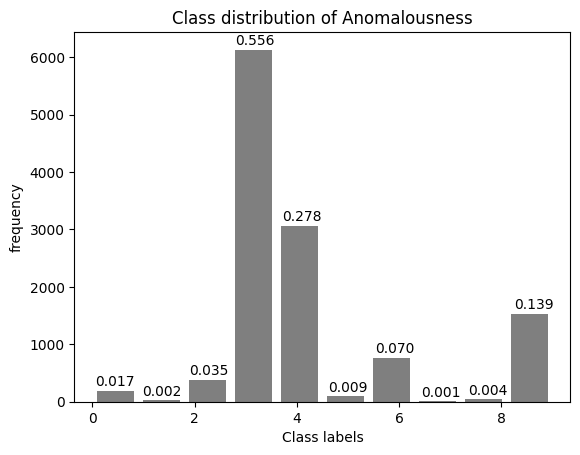
\includegraphics[width=0.5\textwidth]{class_histogram_anomalousness.png}
%\captionof{Histogram of Classification Results\label{fig:classification}}    
\end{center}
The accuracy of the method was 0.65485, or 65.5~\%.



\section{Conclusion}

We were succesful in implementing an active learning algorithm to train a classifier on a dataset of 60000 samples using only a small set of those samples. 
The algorithm was able to reach a 95\% accuracy in far less than 1000 iterations.\par
The SVM classifier performed better than the Random Forest classifier in most cases. 
The highest uncertaintity query strategy was the most effective query strategy for the SVM classifier. 
The lowest vote strategy was the most effective query strategy for the Random Forest classifier. The random query strategy proved to be a quite effective query strategy for both classifiers. 
The entropy query strategy provided mixed results for each classifier.\par
Due to the size of the graphs, they are added to the appendix.
\printbibliography{}
\vspace{12pt}
\end{document}
